\documentclass[11pt]{article}
\usepackage{amsmath, amssymb, array}
\pagestyle{plain}

\textwidth=6.5in
\hoffset-1in
\textheight=9in
\voffset-1in

\usepackage{enumitem}
\usepackage{pgfplots}
\usepackage{graphicx}
\usepackage{lipsum}
\usepackage{stfloats}
\usepackage{multicol}
\usepackage{tikz}
\setlength{\columnsep}{1cm}

\newcommand{\abs}[1]{\left| #1 \right|}


\begin{document}


\noindent MATH 1113   \hspace{1.5in} Worksheet \hspace{1in}   Name \underline{\phantom{alphabetsoupismyveryveryfavorite}}\\ 
\noindent Chapter 1 Challenge \\




\noindent \textbf{Instructions:}  Work together in groups of  3 or 4 to complete the following problems.




\begin{enumerate}
\item Graph the given function and determine how many points need to be plotted to understand the shape of the graph.

\begin{enumerate}
\item $f(x)=-3$, Number of points necessary to plot:  \underline{\phantom{alphabetsoup}}\\
 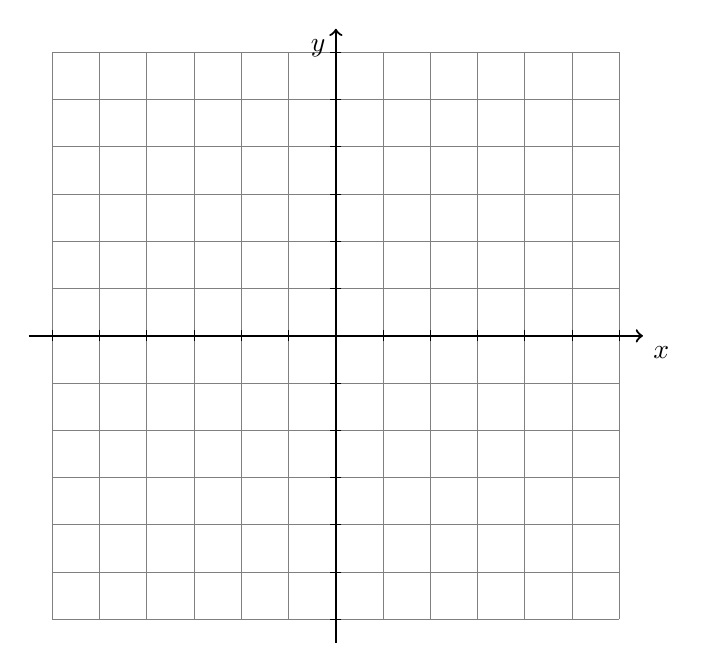
\begin{tikzpicture}[y=.6cm, x=0.6cm,font=\sffamily]
    %% ticks
    \draw[step = 1, gray] (-6,-6) grid (6,6);
    %% axis
    \draw[thick,->] (-6.5,0) -- coordinate (x axis mid) (6.5,0) node[anchor = north west] {$x$};
    \draw[thick,->] (0,-6.5) -- coordinate (y axis mid) (0,6.5) node[anchor = north east] {$y$};
    \foreach \y in {-6,-5,...,-1,1,2,...,6} {
      \draw (2pt, \y) -- (-2pt, \y);
    }
    \foreach \x in {-6,-5,...,-1,1,2,...,6} {
      \draw (\x,2pt) -- (\x,-2pt);
    }

  \end{tikzpicture}

\item $f(x)=x$, Number of points necessary to plot:  \underline{\phantom{alphabetsoup}}\\
 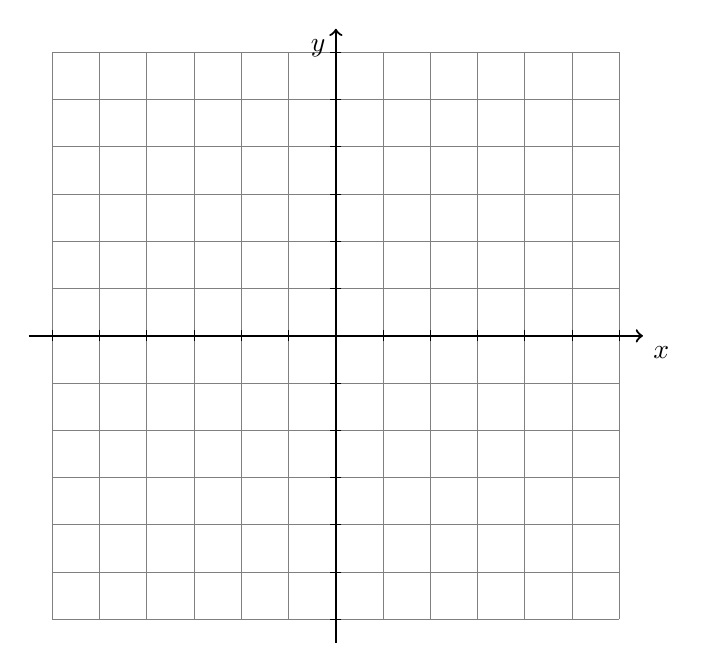
\begin{tikzpicture}[y=.6cm, x=0.6cm,font=\sffamily]
    %% ticks
    \draw[step = 1, gray] (-6,-6) grid (6,6);
    %% axis
    \draw[thick,->] (-6.5,0) -- coordinate (x axis mid) (6.5,0) node[anchor = north west] {$x$};
    \draw[thick,->] (0,-6.5) -- coordinate (y axis mid) (0,6.5) node[anchor = north east] {$y$};
    \foreach \y in {-6,-5,...,-1,1,2,...,6} {
      \draw (2pt, \y) -- (-2pt, \y);
    }
    \foreach \x in {-6,-5,...,-1,1,2,...,6} {
      \draw (\x,2pt) -- (\x,-2pt);
    }

  \end{tikzpicture}

\newpage

\item $f(x)=x^2$, Number of points necessary to plot:  \underline{\phantom{alphabetsoup}}\\
 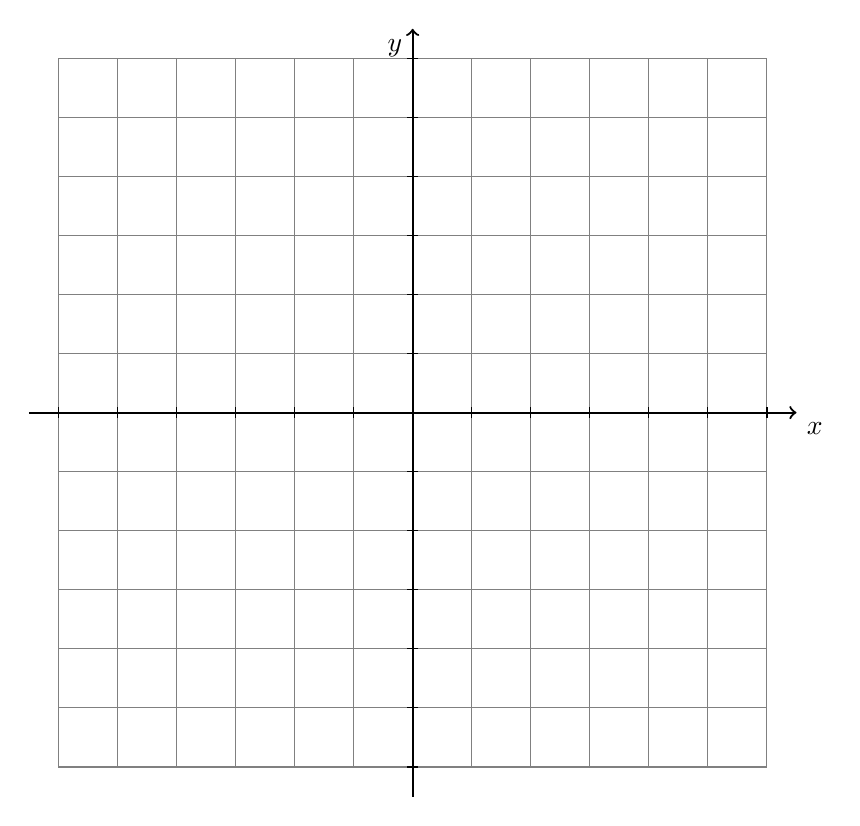
\begin{tikzpicture}[y=.75cm, x=.75cm,font=\sffamily]
    %% ticks
    \draw[step = 1, gray] (-6,-6) grid (6,6);
    %% axis
    \draw[thick,->] (-6.5,0) -- coordinate (x axis mid) (6.5,0) node[anchor = north west] {$x$};
    \draw[thick,->] (0,-6.5) -- coordinate (y axis mid) (0,6.5) node[anchor = north east] {$y$};
    \foreach \y in {-6,-5,...,-1,1,2,...,6} {
      \draw (2pt, \y) -- (-2pt, \y);
    }
    \foreach \x in {-6,-5,...,-1,1,2,...,6} {
      \draw (\x,2pt) -- (\x,-2pt);
    }

  \end{tikzpicture}
  
  
  
  \item $f(x)=x^3$, Number of points necessary to plot:  \underline{\phantom{alphabetsoup}}\\
 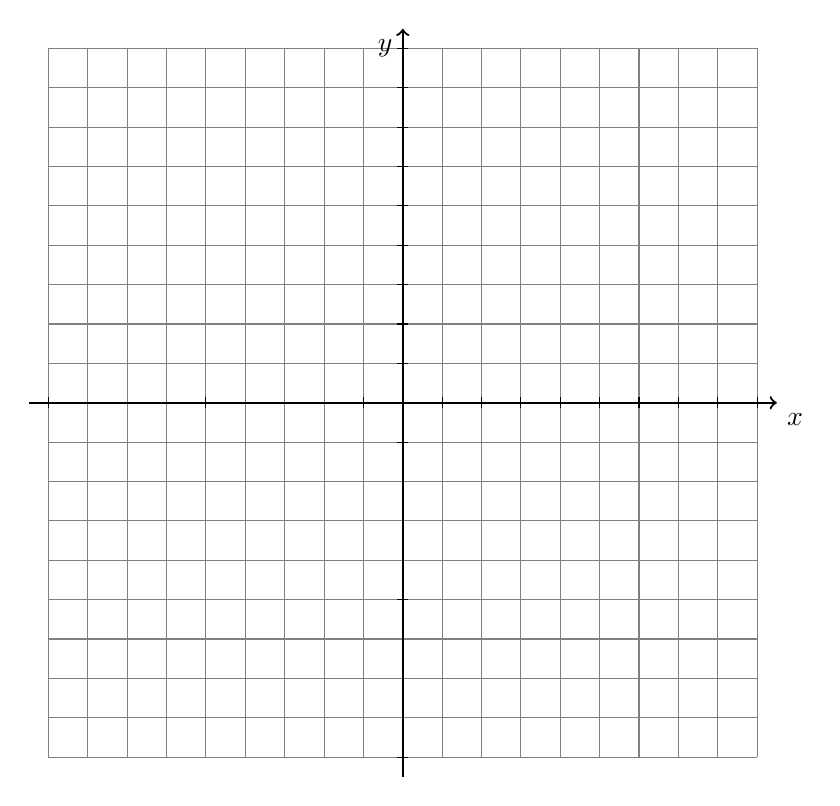
\begin{tikzpicture}[y=.5cm, x=.5cm,font=\sffamily]
    %% ticks
    \draw[step = 1, gray] (-9,-9) grid (9,9);
    %% axis
    \draw[thick,->] (-9.5,0) -- coordinate (x axis mid) (9.5,0) node[anchor = north west] {$x$};
    \draw[thick,->] (0,-9.5) -- coordinate (y axis mid) (0,9.5) node[anchor = north east] {$y$};
    \foreach \y in {-9,-5,...,-1,1,2,...,9} {
      \draw (2pt, \y) -- (-2pt, \y);
    }
    \foreach \x in {-9,-5,...,-1,1,2,...,9} {
      \draw (\x,2pt) -- (\x,-2pt);
    }

  \end{tikzpicture}
  
\vfill

\item $f(x)=\sqrt{x}$, Number of points necessary to plot:  \underline{\phantom{alphabetsoup}}\\
 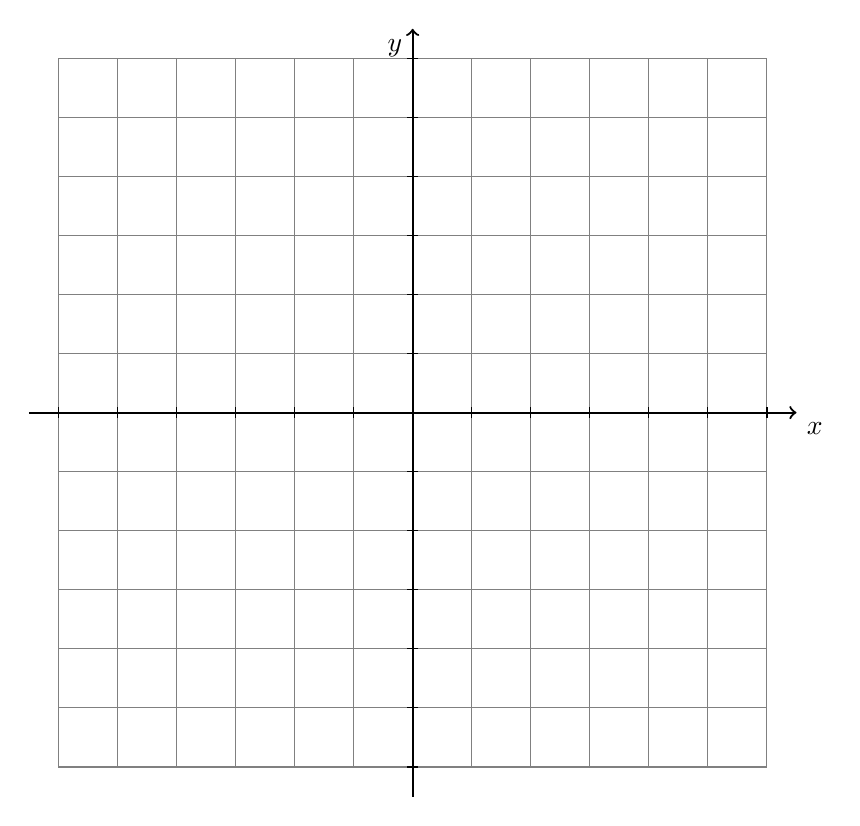
\begin{tikzpicture}[y=.75cm, x=.75cm,font=\sffamily]
    %% ticks
    \draw[step = 1, gray] (-6,-6) grid (6,6);
    %% axis
    \draw[thick,->] (-6.5,0) -- coordinate (x axis mid) (6.5,0) node[anchor = north west] {$x$};
    \draw[thick,->] (0,-6.5) -- coordinate (y axis mid) (0,6.5) node[anchor = north east] {$y$};
    \foreach \y in {-6,-5,...,-1,1,2,...,6} {
      \draw (2pt, \y) -- (-2pt, \y);
    }
    \foreach \x in {-6,-5,...,-1,1,2,...,6} {
      \draw (\x,2pt) -- (\x,-2pt);
    }

  \end{tikzpicture}
  \vfill

\item $f(x)=\sqrt[3]{x}$, Number of points necessary to plot:  \underline{\phantom{alphabetsoup}}\\
 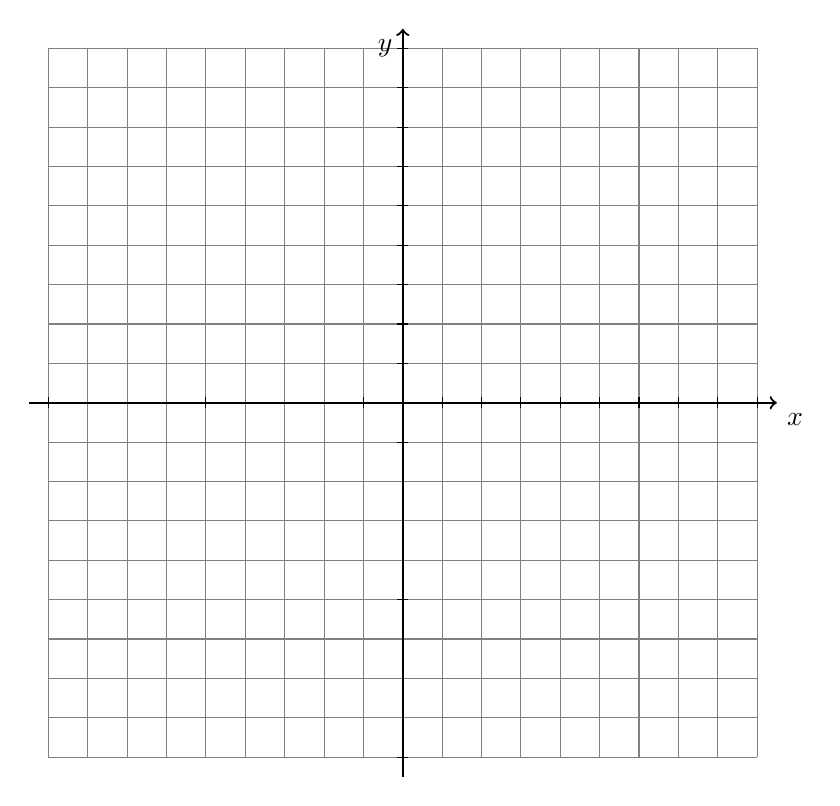
\begin{tikzpicture}[y=.5cm, x=.5cm,font=\sffamily]
    %% ticks
    \draw[step = 1, gray] (-9,-9) grid (9,9);
    %% axis
    \draw[thick,->] (-9.5,0) -- coordinate (x axis mid) (9.5,0) node[anchor = north west] {$x$};
    \draw[thick,->] (0,-9.5) -- coordinate (y axis mid) (0,9.5) node[anchor = north east] {$y$};
    \foreach \y in {-9,-5,...,-1,1,2,...,9} {
      \draw (2pt, \y) -- (-2pt, \y);
    }
    \foreach \x in {-9,-5,...,-1,1,2,...,9} {
      \draw (\x,2pt) -- (\x,-2pt);
    }

  \end{tikzpicture}
\vfill
\newpage

\item $f(x)=|x|$, Number of points necessary to plot:  \underline{\phantom{alphabetsoup}}\\
 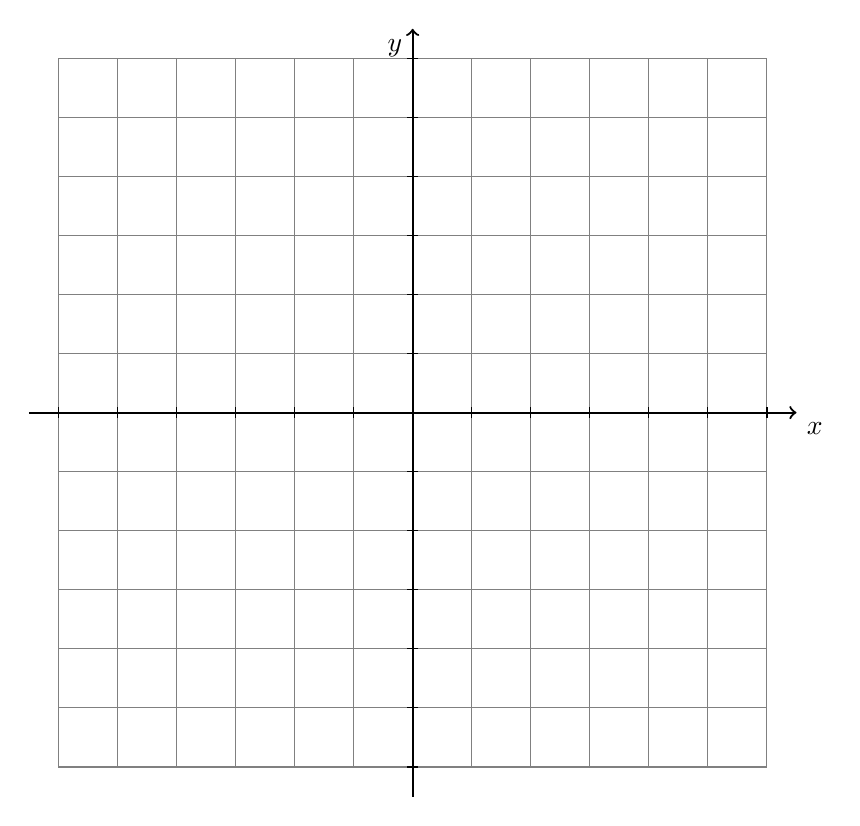
\begin{tikzpicture}[y=.75cm, x=.75cm,font=\sffamily]
    %% ticks
    \draw[step = 1, gray] (-6,-6) grid (6,6);
    %% axis
    \draw[thick,->] (-6.5,0) -- coordinate (x axis mid) (6.5,0) node[anchor = north west] {$x$};
    \draw[thick,->] (0,-6.5) -- coordinate (y axis mid) (0,6.5) node[anchor = north east] {$y$};
    \foreach \y in {-6,-5,...,-1,1,2,...,6} {
      \draw (2pt, \y) -- (-2pt, \y);
    }
    \foreach \x in {-6,-5,...,-1,1,2,...,6} {
      \draw (\x,2pt) -- (\x,-2pt);
    }

  \end{tikzpicture}

\item $\displaystyle f(x)=\frac{1}{x}$, Number of points necessary to plot:  \underline{\phantom{alphabetsoup}}\\
 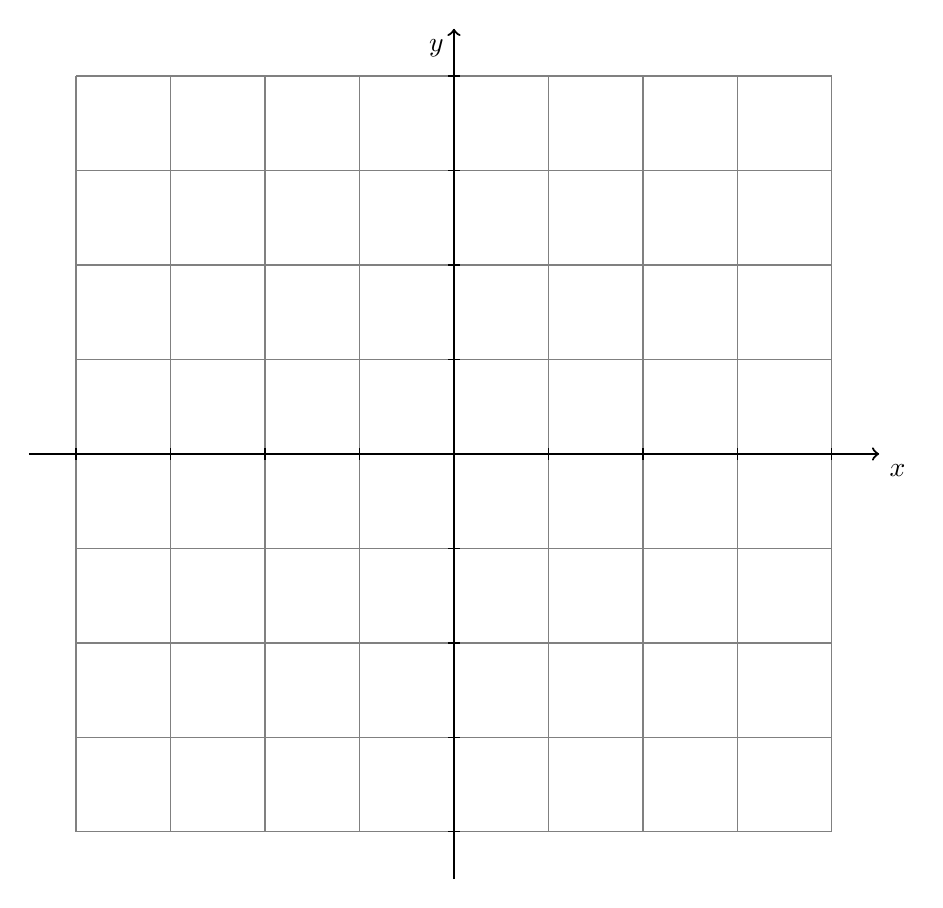
\begin{tikzpicture}[y=1.2cm, x=1.2cm,font=\sffamily]
    %% ticks
    \draw[step = 1, gray] (-4,-4) grid (4,4);
    %% axis
    \draw[thick,->] (-4.5,0) -- coordinate (x axis mid) (4.5,0) node[anchor = north west] {$x$};
    \draw[thick,->] (0,-4.5) -- coordinate (y axis mid) (0,4.5) node[anchor = north east] {$y$};
    \foreach \y in {-4,...,-1,1,2,...,4} {
      \draw (2pt, \y) -- (-2pt, \y);
    }
    \foreach \x in {-4,...,-1,1,2,...,4} {
      \draw (\x,2pt) -- (\x,-2pt);
    }

  \end{tikzpicture}


\end{enumerate}

\newpage

\item Give the coordinates of all of the points that lie on \emph{both} the parabola $y=x^2+1$ \emph{and} the line $y=2x+4$.
	\begin{enumerate}
		\item How can one describe an arbitrary point on the line $y=2x+4$ as an ordered pair?
		\item How can one describe an arbitrary point on the line $y=x^2+1$ as an ordered pair?
		\item How do these descriptions help you find the intersection.
	\end{enumerate}
	
\vspace{2in}		
		
\item Give the coordinates of the four vertices of the square that is contained in Quadrant I and has as two of its vertices the points $(5,0)$ and $(2,4)$.

\vspace{3in}

\item Find the point $(x,y)$ lying on the parabola $y = x^2 + 2x + 1$ so that the average rate of change on the interval between $x$ and $2$ is zero.

\newpage
\item What is the average rate of change on any interval $[x_1,x_2]$ for the linear equation
	$$ax+by+c = 0?$$

\vspace{2in}

\item On the coordinate axes below, draw a function whose domain is
	$$[-2,1]\cup(2,3]\cup\{5\}$$
	and whose range is
	$$[-6,-4)\cup[-1,1]\cup\{2\}\cup(3,4].$$

\begin{center}
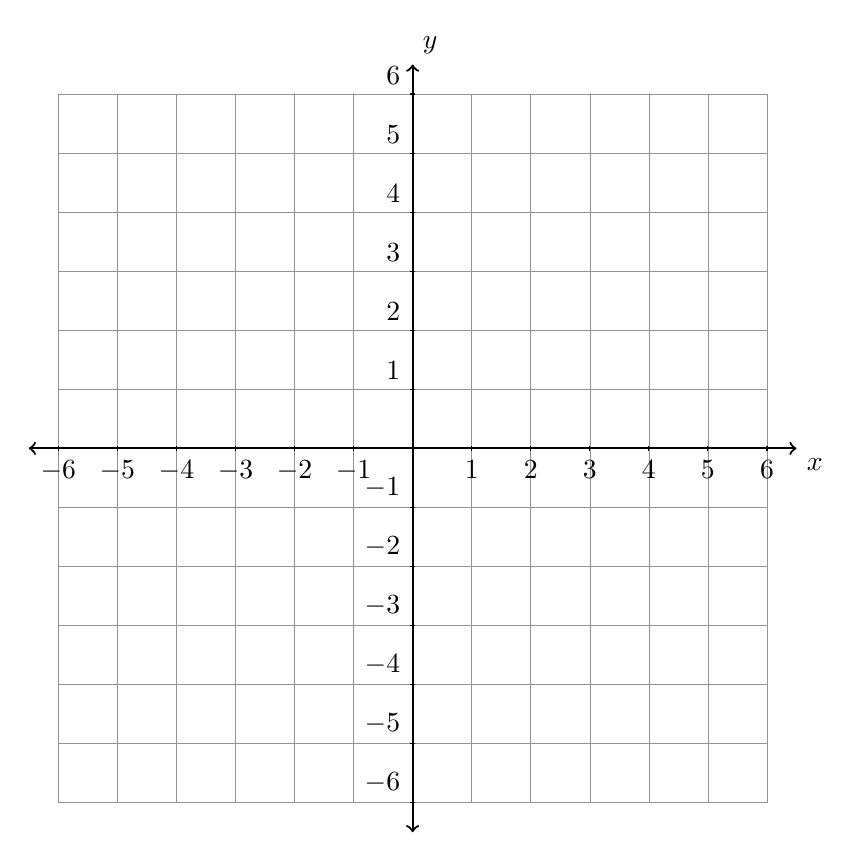
\begin{tikzpicture}[y=.75cm, x=.75cm,font=\sffamily,
	mydot/.style={
    circle,
    fill=white,
    draw,
    outer sep=0pt,
    inner sep=1.5pt
    }]
    %% Add a grid
    \draw[step = 1, gray, very thin,opacity=0.85] (-6, -6) grid ( 6, 6);
 	%% Draw the axes
	\draw[thick,<->] (-6.5,0) -- coordinate (x axis mid) (6.5,0) node[anchor = north west] {$x$};
    \draw[thick,<->] (0,-6.5) -- coordinate (y axis mid) (0,6.5) node[anchor = south west] {$y$};
    %% Label the y axis
    \foreach \y in {-6,...,-1,1,2,...,6} {
    	\draw (1pt, \y) -- (-1pt, \y) node[anchor = south east] {$\y$};
    }
    %% Label the x axis
    \foreach \x in {-6,...,-1,1,2,...,6} {
    	\draw (\x,1pt) -- (\x,-1pt) node[anchor = north] {$\x$};
    }
    %% Draw the function.
%    \begin{scope}
%         \draw[scale=1.0,very thick,black] (-2, 0) -- (1,-2);
%         \draw[scale=1.0,very thick,black] (1.05,1.04) -- (3,2);
%         \fill[black] (-2, 0) circle[radius=0.5ex];
%         \fill[black] (3,2) circle[radius=0.5ex];
%         \fill[black] (1,-2) circle[radius=0.5ex];
%         \draw[scale=1.0, very thick, black] (1,1) circle[radius=0.5ex];
%    \end{scope}

    %%\node[above=0.1cm] at (-2,2 )   {\nextXValue};

\end{tikzpicture}
\end{center}



\end{enumerate}

















\end{document}